\subsection{Probe 1}

Die erste Probe zeigt eine gleichmäßige, klar abgegrenzte Struktur mit regelmäßig angeordneten quadratischen Elementen (siehe Abbildung~\ref{Abbildung 6 :probe1}). Die Reflexionssignale erscheinen homogen, ohne sichtbare Unterbrechungen oder Unregelmäßigkeiten innerhalb der Materialübergänge. Auffällig ist die hohe Signalklarheit in den bondfreien Zonen. Es lassen sich weder Risse noch Delaminationen erkennen, was auf eine saubere Verarbeitung und intakte Schichten schließen lässt.
\vspace{0.2cm}
\begin{figure}[htbp]
    \centering
    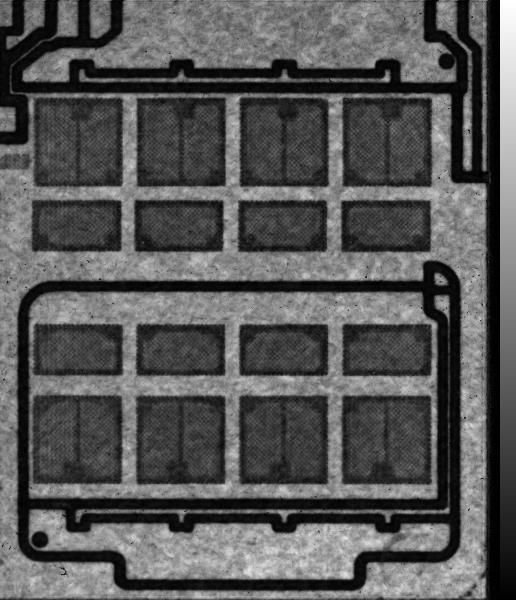
\includegraphics[scale=0.20]{Bilder/Probe11.jpg}
    \caption{C-Scan der Probe 1 mit klar erkennbaren Strukturen und homogener Reflexion.}
    \label{Abbildung 6 :probe1}
\end{figure}
\begin{figure}[htbp]
    \centering
    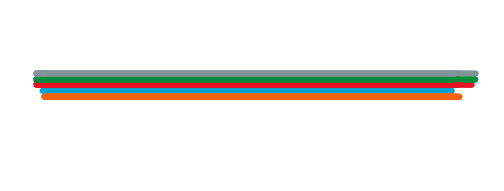
\includegraphics[scale=0.75]{Bilder/probelinie1}
    \caption{Schematische Darstellung der Materialschichten der Probe 1 (DCB-Modul) mit farblich gekennzeichneten Ebenen. Die grüne Linie stellt den gesinterten Halbleiter dar, die rote Linie die Bondschicht, die blaue Linie das Keramiksubstrat und die orange Linie die Kupferbasis.}
    \label{Abbildung 7 :Schematische Darstellung der Materialschichten der Probe 1 (DCB-Modul) mit farblich gekennzeichneten Ebenen. Die grüne Linie stellt den gesinterten Halbleiter dar, die rote Linie die Bondschicht, die blaue Linie das Keramiksubstrat und die orange Linie die Kupferbasis.}
\end{figure}
\vspace{0.5cm}
\subsection{Probe 2}
An Probe 2 wird eine schichtweise Analyse durchgeführt. In den insgesamt fünf gewählten Fokusebenen zeigen sich deutliche Unterschiede in Signalintensität und den erkennbaren Strukturen. Die obersten Bildebenen (Abbildung 8, obere Aufnahmen) wirken relativ glatt und homogen. Allerdings ist bereits hier eine kreisförmige Auffälligkeit in Form eines dunklen Spots zu erkennen. Diese runde dunkle Stelle sticht in der rechten Abbildung 8 deutlich hervor und könnte auf einen Lufteinschluss oder eine lokale Delamination direkt unter der Metalloberfläche hindeuten. Möglich ist, dass sich an dieser Stelle eine kleine Luftblase im Schweißpunkt gebildet hat oder die Verbindung zum Substrat nicht vollflächig gelingt. Mit zunehmender Tiefe (Abbildungen 9) treten mehr Leiterstrukturen hervor, die in den oberen Schichten noch nicht sichtbar sind. Insbesondere werden die im Kupfer-Leadframe eingebetteten Leiterbahnen und Bondflächen in den mittleren Ebenen klarer erkennbar. In den tieferen Fokusebenen (Abbildung 10, tiefste Ebene) zeigen sich zudem feine Schattenbildungen und leichte Signalunterbrechungen entlang einzelner Linienstrukturen. Diese Unregelmäßigkeiten konzentrieren sich vor allem im unteren Bildbereich der Abbildung 10, wo Bond- oder Kontaktzonen zum Keramiksubstrat verlaufen. Das deutet darauf hin, dass in den unteren Schichten etwa an der Grenzfläche zwischen einer Bondschicht und dem Substrat Stellen mit geringerer akustischer Kopplung vorhanden sind. Mögliche Ursachen dafür sind Mikrorisse in der Bond bzw. Lötverbindung. Eine solche Schwachstelle in der Materialanbindung ruft genau solche lokalen Abschwächungen im Reflexionssignal hervor. Auch der Umstand, dass die Probe im Scan leicht geneigt ist (siehe unterschiedliche Schärfe in den Bildecken), kann zu kleinen Helligkeitsunterschieden beitragen, erklärt jedoch nicht vollständig die beobachteten Schatten entlang der Leiterbahnen. Insgesamt weist Probe 2 damit auf vereinzelte Defizite in der Schweißverbindung hin, ein potenzieller Lufteinschluss nahe der Oberfläche und mögliche Delaminationen in tieferen Bondschichten. Diese Defekte entstehen durch ungleichmäßiges Aufschweißen des Kupfers auf die Keramik, durch unzureichenden Druck oder Verunreinigungen beim Fügen, und führen langfristig möglicherweise zu thermischen Problemen oder mechanischer Instabilität.
\vspace{0.2cm}
\begin{figure}[htbp]
    \centering
    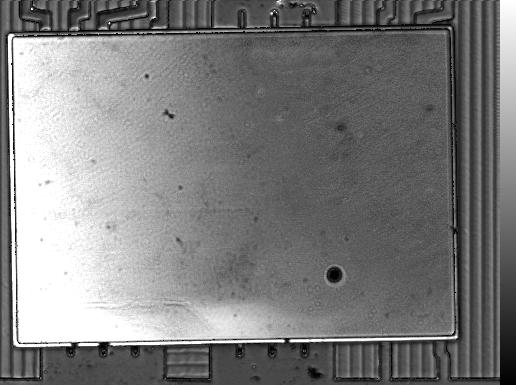
\includegraphics[scale=0.30]{Bilder/Probe2_i794_x001.jpg}
    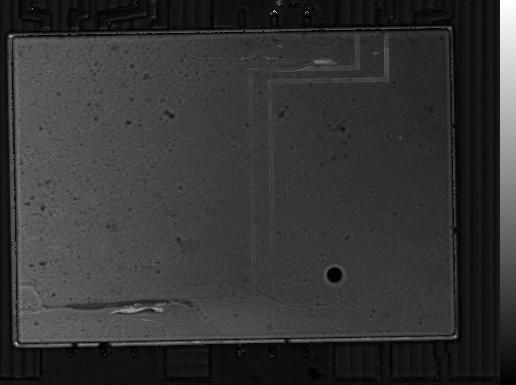
\includegraphics[scale=0.30]{Bilder/Probe2_i794_x002.jpg}
    \caption{Obere Fokusebenen der Probe 2. Die rechte Abbildung zeigt eine auffällige Reflexionsunterbrechung.}
    \label{Abbildung 8_1:probe2_1}
    \label{Abbildung 8_2:probe2_2}
\end{figure}

\begin{figure}[H]
    \centering
    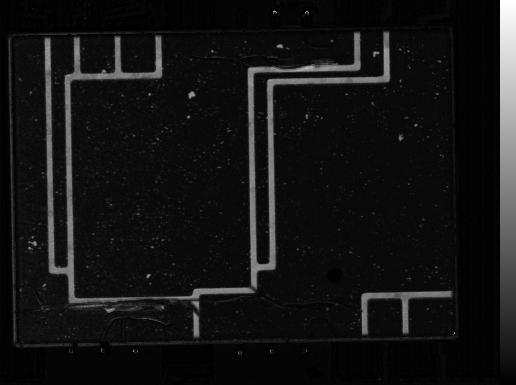
\includegraphics[scale=0.30]{Bilder/Probe2_i794_x003.jpg}
    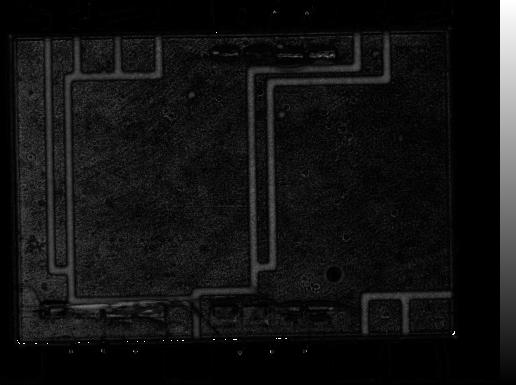
\includegraphics[scale=0.30]{Bilder/Probe2_i794_x004.jpg}
    \caption{Mittlere Fokusebenen der Probe 2 mit zunehmender Sichtbarkeit der Leiterstrukturen.}
    \label{Abbildung 9_1:probe2_3}
    \label{Abbildung 9_2:probe2_4}
\end{figure}

\begin{figure}[H]
    \centering
    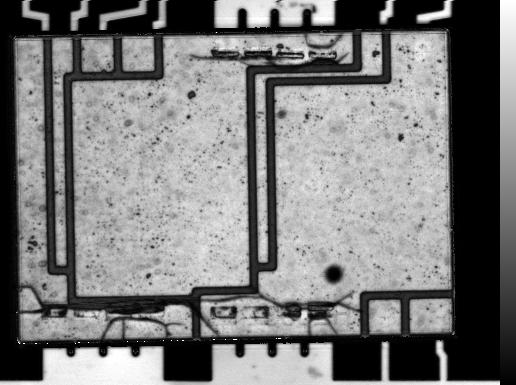
\includegraphics[scale=0.30]{Bilder/Probe2_i794_x005.jpg}
    \caption{Tiefste gescannte Ebene der Probe 2. Sichtbare Leiterbahnen mit lokalen Unregelmäßigkeiten im unteren Bereich.}
    \label{Abbildung 10:probe2_5}
\end{figure}
\begin{figure}[H]
    \centering
    
\includegraphics[scale=0.75]{Bilder/probelinie2}
    \caption{Visualisierung der in mehreren Fokusebenen gescannten Schichten der Probe 2. Die graue Linie zeigt die Oberfläche bzw. Metallabdeckung, die roten Linien markieren Bond- oder Kontaktzonen, die orange Linie kennzeichnet Kupferleiterbahnen, und die blaue Linie stellt das keramische Substrat dar.}
    \label{Abbildung 11 :Visualisierung der in mehreren Fokusebenen gescannten Schichten der Probe 2. Die graue Linie zeigt die Oberfläche bzw. Metallabdeckung, die roten Linien markieren Bond- oder Kontaktzonen, die orange Linie kennzeichnet Kupferleiterbahnen, und die blaue Linie stellt das keramische Substrat dar.}
\end{figure}

\subsection{Probe 3}

In der letzten Probe, einem DoL-Modul, fällt sofort die großflächige, glatte Reflexionsfläche auf (siehe Abbildung~\ref{Abbildung 12:probe3}). Bemerkenswert ist jedoch die gute Lesbarkeit des Schriftzugs \enquote{FH-KIEL} in der Bildmitte. Die klare Abbildung des Schriftzugs lässt darauf schließen, dass auf der Oberfläche des Moduls eine Gravur oder Markierung vorhanden ist, welche die akustische Reflexion lokal beeinflusst. Die gleichmäßige Reflexion dieser Gravur weist auf eine intakte, gleichmäßig metallisierte Oberfläche hin. Kleinere Unregelmäßigkeiten in Form dunkler Punkte oder Flecken lassen sich lediglich vereinzelt beobachten. Dabei handelt es sich höchstwahrscheinlich um minimale Oberflächenverunreinigungen oder mikroskopisch kleine Lufteinschlüsse, die die Gesamtstruktur jedoch nicht wesentlich beeinträchtigen. Auch in tieferen Schichten etwa in der organischen Trägerfolie oder den eingebetteten Kupferstrukturen zeigen sich keine auffälligen Defekte oder Störungen. Das akustische Bild bleibt über die gesamte Fläche hinweg konsistent. Die Tatsache, dass selbst feine Gravuren wie „FH-KIEL“ deutlich sichtbar sind, unterstreicht die hohe Empfindlichkeit und Auflösung des gewählten Scanverfahrens. Insgesamt weist Probe 3 somit auf einen sehr homogenen Schichtaufbau hin. Die gleichmäßige Verbindung zwischen Kupferstruktur und Folie sowie die fehlenden Delaminationen oder Risse deuten auf eine stabile und qualitativ hochwertige Materialanbindung hin, die für den Einsatz in der Leistungselektronik von entscheidender Bedeutung ist.
\vspace{0.2cm}
\begin{figure}[H]
    \centering
    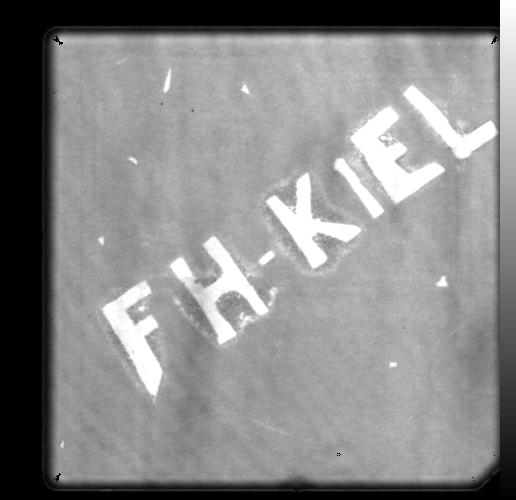
\includegraphics[scale=0.30]{Bilder/Probe3_i795_c.jpg}
    \caption{C-Scan der Probe 3 (DoL-Modul) mit gleichmäßiger Reflexionsfläche und klar erkennbarer Gravurstruktur.}
    \label{Abbildung 12:probe3}
\end{figure}
\vspace{0.2cm}
\begin{figure}[H]
    \centering
    
\includegraphics[scale=0.75]{Bilder/probelinie3}
    \caption{Schichtdarstellung der Probe 3 (DoL-Modul) mit farblich codierten Materialien. Die graue Linie stellt die Oberfläche bzw. die Beschriftung dar, die schwarze Linie die Metallkappe, die violette Linie steht für die organische Trägerfolie und die orange Linie kennzeichnet die eingebetteten Kupferstrukturen.}
    \label{Abbildung 13 :Schichtdarstellung der Probe 3 (DoL-Modul) mit farblich codierten Materialien. Die schwarze Linie stellt die Metallkappe dar, die violette Linie steht für die organische Trägerfolie und die orange Linie kennzeichnet die eingebetteten Kupferstrukturen.}
\end{figure}